\section{Reta}

Uma reta guarda a direção \texttt{v} e a constante \texttt{c}: são os pontos $p$ com \texttt{cross(v, p)} $= c$.
Dá para criar por dois pontos \texttt{line(p, q)} (direção $q - p$), por direção e constante \texttt{line(v, c)} ou
pela equação $ax + by = c$ com \texttt{line(a, b, c)}.

\subsection*{Lado, distância, projeção e reflexão}

\smallskip{\centering
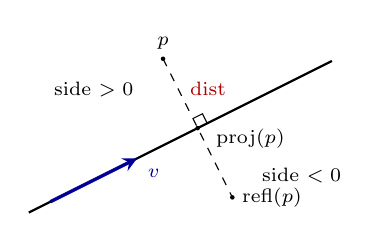
\begin{tikzpicture}[scale=0.55, >=stealth]
  \draw[thick] (-0.5,-0.25) -- (6.5,3.25);
  \draw[->, very thick, blue!60!black] (0,0) -- (2,1) node[below right] {\scriptsize $v$};
  \fill (2.6,3.3) circle (1.5pt) node[above] {\scriptsize $p$};
  \fill (3.4,1.7) circle (1.5pt);
  \node[right] at (3.6,1.45) {\scriptsize proj$(p)$};
  \fill (4.2,0.1) circle (1.5pt) node[right] {\scriptsize refl$(p)$};
  \draw[dashed] (2.6,3.3) -- (4.2,0.1);
  \draw (3.62,1.81) -- (3.51,2.03) -- (3.29,1.92);
  \node[red!70!black, right] at (3.0,2.6) {\scriptsize dist};
  \node at (1.0,2.6) {\scriptsize side $> 0$};
  \node at (5.8,0.6) {\scriptsize side $< 0$};
\end{tikzpicture}
\par}\smallskip

\begin{itemize}
  \item \texttt{side(p)} $=$ \texttt{cross(v, p)} $- c$: positivo se $p$ está à esquerda de $v$, negativo à
        direita e zero na reta. Vale $|v|$ vezes a distância com sinal, e é exato com \texttt{T} inteiro.
  \item \texttt{dist(p)} $= |\text{side}(p)| / |v|$, a distância de $p$ até a reta.
  \item \texttt{proj(p)} é o ponto da reta mais perto de $p$, e \texttt{refl(p)} é o espelho de $p$ pela reta
        (o dobro do caminho até a projeção).
  \item \texttt{comp(p, q)} diz se $p$ vem antes de $q$ andando no sentido de $v$, comparando as projeções.
        Serve para ordenar pontos ao longo da reta.
\end{itemize}

\subsection*{Perpendicular, paralela e deslocamento}

\smallskip{\centering
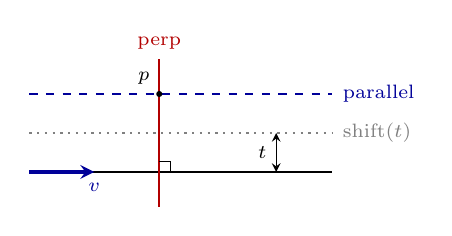
\begin{tikzpicture}[scale=0.55, >=stealth]
  \draw[thick] (-0.5,0) -- (6.5,0);
  \draw[->, very thick, blue!60!black] (-0.5,0) -- (1,0) node[below] {\scriptsize $v$};
  \draw[blue!60!black, dashed, thick] (-0.5,1.8) -- (6.5,1.8) node[right] {\scriptsize parallel};
  \draw[red!70!black, thick] (2.5,-0.8) -- (2.5,2.6) node[above] {\scriptsize perp};
  \fill (2.5,1.8) circle (2pt) node[above left] {\scriptsize $p$};
  \draw (2.5,0.25) -- (2.75,0.25) -- (2.75,0);
  \draw[gray, dotted, thick] (-0.5,0.9) -- (6.5,0.9) node[right] {\scriptsize shift$(t)$};
  \draw[<->] (5.2,0) -- (5.2,0.9) node[midway, left] {\scriptsize $t$};
\end{tikzpicture}
\par}\smallskip

\texttt{perp\_through(p)} é a reta por $p$ que faz $90^\circ$ com esta, e \texttt{parallel\_through(p)} é a reta por
$p$ com a mesma direção; as duas são exatas com \texttt{T} inteiro. \texttt{shift(t)} desloca a reta $t$ para a
esquerda de $v$ (para a direita se $t < 0$), útil para faixas de largura fixa; exige \texttt{T} real.

\subsection*{Interseções}

\smallskip{\centering
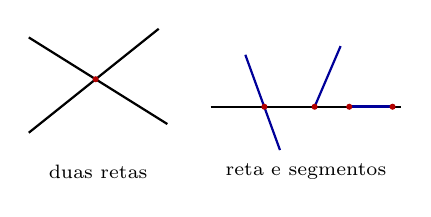
\begin{tikzpicture}[scale=0.55, >=stealth]
  \draw[thick] (0,0) -- (3,2.4);
  \draw[thick] (0,2.2) -- (3.2,0.2);
  \fill[red!70!black] (1.544,1.235) circle (2pt);
  \node at (1.6,-0.9) {\scriptsize duas retas};
  \draw[thick] (4.2,0.6) -- (8.6,0.6);
  \draw[blue!60!black, thick] (5.0,1.8) -- (5.8,-0.4);
  \fill[red!70!black] (5.44,0.6) circle (2pt);
  \draw[blue!60!black, thick] (6.6,0.6) -- (7.2,2.0);
  \fill[red!70!black] (6.6,0.6) circle (2pt);
  \draw[blue!60!black, very thick] (7.4,0.6) -- (8.4,0.6);
  \fill[red!70!black] (7.4,0.6) circle (2pt);
  \fill[red!70!black] (8.4,0.6) circle (2pt);
  \node at (6.4,-0.9) {\scriptsize reta e segmentos};
\end{tikzpicture}
\par}\smallskip

\texttt{line\_inter(l, r)} devolve o ponto de encontro, ou vazio se as retas são paralelas.
\texttt{line\_segment\_inter(l, a, b)} devolve onde o segmento $[a, b]$ corta a reta: vazio se as pontas estão do
mesmo lado, um ponto se ele atravessa ou só encosta, e as duas pontas se o segmento está em cima da reta.

\textbf{Exato ou real.} \texttt{side}, \texttt{dist}, \texttt{comp}, \texttt{perp\_through} e
\texttt{parallel\_through} funcionam com \texttt{T} inteiro. \texttt{shift}, \texttt{proj}, \texttt{refl} e as
interseções exigem \texttt{T} real (têm \texttt{assert}).
